\documentclass[11pt,a4paper]{ctexart}
% Shared preamble for the assignment reports. Use with:
%   \documentclass[11pt,a4paper]{ctexart}  (XeLaTeX)
%   % Shared preamble for the assignment reports. Use with:
%   \documentclass[11pt,a4paper]{ctexart}  (XeLaTeX)
%   % Shared preamble for the assignment reports. Use with:
%   \documentclass[11pt,a4paper]{ctexart}  (XeLaTeX)
%   \input{../common/preamble.tex}
\usepackage[margin=2.3cm]{geometry}
\setmainfont{texgyretermes}[Extension=.otf,UprightFont=*-regular,BoldFont=*-bold,ItalicFont=*-italic,BoldItalicFont=*-bolditalic]
\setsansfont{texgyreheros}[Extension=.otf,UprightFont=*-regular,BoldFont=*-bold,ItalicFont=*-italic,BoldItalicFont=*-bolditalic]
\setmonofont{texgyrecursor}[Extension=.otf,UprightFont=*-regular,BoldFont=*-bold,ItalicFont=*-italic,BoldItalicFont=*-bolditalic]
\usepackage{amsmath,amssymb,mathtools,bm}
\usepackage{graphicx}
\usepackage{booktabs,multirow,makecell,array,tabularx}
\usepackage[table]{xcolor}
\usepackage[most]{tcolorbox}
\usepackage{enumitem}
\usepackage{listings}
\usepackage{subcaption}
\usepackage{siunitx}
\usepackage[hidelinks]{hyperref}
\usepackage[nameinlink,noabbrev]{cleveref}
\usepackage{float}

\setlength{\emergencystretch}{3em}
\linespread{1.15}
\setlist{leftmargin=*,itemsep=2pt,topsep=3pt}
\graphicspath{{figures/}}

\crefname{figure}{图}{图}
\crefname{table}{表}{表}
\crefname{section}{第}{第}
\creflabelformat{section}{#2#1#3 节}
\crefname{equation}{式}{式}
\crefformat{equation}{式~(#2#1#3)}

\lstset{basicstyle=\ttfamily\footnotesize,columns=fullflexible,breaklines=true,frame=single,
  framerule=0.3pt,rulecolor=\color{black!40},backgroundcolor=\color{black!3},
  keywordstyle=\color{blue!60!black}\bfseries,commentstyle=\color{green!40!black},
  numbers=left,numberstyle=\tiny\color{black!50},xleftmargin=1.5em}

% Interview boxes: question, model answer, common wrong answer.
\newtcolorbox{iqbox}[1]{enhanced,breakable,colback=blue!3,colframe=blue!45!black,boxrule=0.5pt,arc=1.5pt,
  left=4pt,right=4pt,top=3pt,bottom=3pt,fonttitle=\bfseries\small,title={面试追问：#1}}
\newtcolorbox{findingbox}[1][]{enhanced,breakable,colback=green!3,colframe=green!40!black,boxrule=0.5pt,arc=1.5pt,
  left=4pt,right=4pt,top=3pt,bottom=3pt,fonttitle=\bfseries\small,title={结论#1}}
\newtcolorbox{caveatbox}{enhanced,breakable,colback=orange!4,colframe=orange!60!black,boxrule=0.5pt,arc=1.5pt,
  left=4pt,right=4pt,top=3pt,bottom=3pt,fonttitle=\bfseries\small,title={不能推出的结论}}

\newcommand{\authorline}{ShaneLiu04\thanks{GitHub: \url{https://github.com/ShaneLiu04}。代码与原始指标见 edge-deploy 仓库各 lab 的 \texttt{artifacts/raw/}。本文基于公开课程材料独立完成，与课程团队无隶属关系。}}

\usepackage[margin=2.3cm]{geometry}
\setmainfont{texgyretermes}[Extension=.otf,UprightFont=*-regular,BoldFont=*-bold,ItalicFont=*-italic,BoldItalicFont=*-bolditalic]
\setsansfont{texgyreheros}[Extension=.otf,UprightFont=*-regular,BoldFont=*-bold,ItalicFont=*-italic,BoldItalicFont=*-bolditalic]
\setmonofont{texgyrecursor}[Extension=.otf,UprightFont=*-regular,BoldFont=*-bold,ItalicFont=*-italic,BoldItalicFont=*-bolditalic]
\usepackage{amsmath,amssymb,mathtools,bm}
\usepackage{graphicx}
\usepackage{booktabs,multirow,makecell,array,tabularx}
\usepackage[table]{xcolor}
\usepackage[most]{tcolorbox}
\usepackage{enumitem}
\usepackage{listings}
\usepackage{subcaption}
\usepackage{siunitx}
\usepackage[hidelinks]{hyperref}
\usepackage[nameinlink,noabbrev]{cleveref}
\usepackage{float}

\setlength{\emergencystretch}{3em}
\linespread{1.15}
\setlist{leftmargin=*,itemsep=2pt,topsep=3pt}
\graphicspath{{figures/}}

\crefname{figure}{图}{图}
\crefname{table}{表}{表}
\crefname{section}{第}{第}
\creflabelformat{section}{#2#1#3 节}
\crefname{equation}{式}{式}
\crefformat{equation}{式~(#2#1#3)}

\lstset{basicstyle=\ttfamily\footnotesize,columns=fullflexible,breaklines=true,frame=single,
  framerule=0.3pt,rulecolor=\color{black!40},backgroundcolor=\color{black!3},
  keywordstyle=\color{blue!60!black}\bfseries,commentstyle=\color{green!40!black},
  numbers=left,numberstyle=\tiny\color{black!50},xleftmargin=1.5em}

% Interview boxes: question, model answer, common wrong answer.
\newtcolorbox{iqbox}[1]{enhanced,breakable,colback=blue!3,colframe=blue!45!black,boxrule=0.5pt,arc=1.5pt,
  left=4pt,right=4pt,top=3pt,bottom=3pt,fonttitle=\bfseries\small,title={面试追问：#1}}
\newtcolorbox{findingbox}[1][]{enhanced,breakable,colback=green!3,colframe=green!40!black,boxrule=0.5pt,arc=1.5pt,
  left=4pt,right=4pt,top=3pt,bottom=3pt,fonttitle=\bfseries\small,title={结论#1}}
\newtcolorbox{caveatbox}{enhanced,breakable,colback=orange!4,colframe=orange!60!black,boxrule=0.5pt,arc=1.5pt,
  left=4pt,right=4pt,top=3pt,bottom=3pt,fonttitle=\bfseries\small,title={不能推出的结论}}

\newcommand{\authorline}{ShaneLiu04\thanks{GitHub: \url{https://github.com/ShaneLiu04}。代码与原始指标见 edge-deploy 仓库各 lab 的 \texttt{artifacts/raw/}。本文基于公开课程材料独立完成，与课程团队无隶属关系。}}

\usepackage[margin=2.3cm]{geometry}
\setmainfont{texgyretermes}[Extension=.otf,UprightFont=*-regular,BoldFont=*-bold,ItalicFont=*-italic,BoldItalicFont=*-bolditalic]
\setsansfont{texgyreheros}[Extension=.otf,UprightFont=*-regular,BoldFont=*-bold,ItalicFont=*-italic,BoldItalicFont=*-bolditalic]
\setmonofont{texgyrecursor}[Extension=.otf,UprightFont=*-regular,BoldFont=*-bold,ItalicFont=*-italic,BoldItalicFont=*-bolditalic]
\usepackage{amsmath,amssymb,mathtools,bm}
\usepackage{graphicx}
\usepackage{booktabs,multirow,makecell,array,tabularx}
\usepackage[table]{xcolor}
\usepackage[most]{tcolorbox}
\usepackage{enumitem}
\usepackage{listings}
\usepackage{subcaption}
\usepackage{siunitx}
\usepackage[hidelinks]{hyperref}
\usepackage[nameinlink,noabbrev]{cleveref}
\usepackage{float}

\setlength{\emergencystretch}{3em}
\linespread{1.15}
\setlist{leftmargin=*,itemsep=2pt,topsep=3pt}
\graphicspath{{figures/}}

\crefname{figure}{图}{图}
\crefname{table}{表}{表}
\crefname{section}{第}{第}
\creflabelformat{section}{#2#1#3 节}
\crefname{equation}{式}{式}
\crefformat{equation}{式~(#2#1#3)}

\lstset{basicstyle=\ttfamily\footnotesize,columns=fullflexible,breaklines=true,frame=single,
  framerule=0.3pt,rulecolor=\color{black!40},backgroundcolor=\color{black!3},
  keywordstyle=\color{blue!60!black}\bfseries,commentstyle=\color{green!40!black},
  numbers=left,numberstyle=\tiny\color{black!50},xleftmargin=1.5em}

% Interview boxes: question, model answer, common wrong answer.
\newtcolorbox{iqbox}[1]{enhanced,breakable,colback=blue!3,colframe=blue!45!black,boxrule=0.5pt,arc=1.5pt,
  left=4pt,right=4pt,top=3pt,bottom=3pt,fonttitle=\bfseries\small,title={面试追问：#1}}
\newtcolorbox{findingbox}[1][]{enhanced,breakable,colback=green!3,colframe=green!40!black,boxrule=0.5pt,arc=1.5pt,
  left=4pt,right=4pt,top=3pt,bottom=3pt,fonttitle=\bfseries\small,title={结论#1}}
\newtcolorbox{caveatbox}{enhanced,breakable,colback=orange!4,colframe=orange!60!black,boxrule=0.5pt,arc=1.5pt,
  left=4pt,right=4pt,top=3pt,bottom=3pt,fonttitle=\bfseries\small,title={不能推出的结论}}

\newcommand{\authorline}{ShaneLiu04\thanks{GitHub: \url{https://github.com/ShaneLiu04}。代码与原始指标见 edge-deploy 仓库各 lab 的 \texttt{artifacts/raw/}。本文基于公开课程材料独立完成，与课程团队无隶属关系。}}

\graphicspath{{../../solutions/mit6.5940/lab1-pruning/artifacts/figures/}{../../solutions/mit6.5940/lab2-vgg/artifacts/figures/}{../../solutions/mit6.5940/lab4-awq/artifacts/figures/}{../../solutions/mit6.5940/lab5-tinychat/artifacts/figures/}}

\title{MIT 6.5940 Fall 2024 实验报告：\\剪枝、k-means 与整数量化、AWQ、W4A8 kernel}
\author{\authorline}
\date{2026 年 11 月}

\begin{document}
\maketitle

\begin{abstract}
本报告覆盖 MIT 6.5940（TinyML and Efficient Deep Learning，Song Han，Fall 2024）的 Lab 1、Lab 2（官方 VGG 题）、Lab 4 与 Lab 5；Lab 3（NAS）与期末项目单独成文。
实现全部独立编写，不复制官方 notebook；数据与协议与课程一致。
主要结论：
（a）Lab 1：按敏感度为 9 层选稀疏度，VGG 只剩 23.6\% 尺寸，5 轮微调回到 92.72\%（要求 $\le$25\%、$\ge$92.5\%）；通道剪 30\% 时 MACs 0.504 倍、单线程延迟 0.64 倍、微调后 92.52\%；
（b）Lab 2：k-means 8 / 4 / 2 bit 经 QAT 分别为 92.82 / 92.84 / 92.18\%；整数 int8 VGG 92.94\%，与 fp32 的 92.95\% 只差 1 张图；
（c）Lab 4：OPT-1.3B 的 W3 g128 RTN 困惑度 107.97，按激活保留 1\% 通道为 fp16 是 16.69，按权重或随机保留 1\% 都在 100 以上；AWQ 不保留任何 fp16 通道做到 16.87，加截断 16.04；
（d）Lab 5：TinyChatEngine 的 W4A8 GEMM 六个实现全部通过官方正确性检查，四种技术合用比参考实现快 28.2 倍（26.09 对 0.92 GOP/s），LLaMA2-7B 端到端 decode 快 12.5 倍；把课程 Makefile 的 \texttt{-O0} 换成 \texttt{-O3}，kernel 差距拉大到 51.5 倍，端到端 191 ms/token。
\end{abstract}

\tableofcontents
\newpage

\section{Lab 1：剪枝}\label{sec:lab1}

\subsection{设置}
课程 VGG（8 个 3$\times$3 卷积 + BN + ReLU，4 次最大池化，全局平均池化后 512$\to$10 的线性层），课程预训练权重在 CIFAR-10 测试集上 92.95\%，fp32 共 9,228,362 个参数、35.20 MiB。
数据只做 \texttt{ToTensor}；训练增强是 RandomCrop(32, pad 4) 与水平翻转，在 GPU 上逐样本完成。微调统一用课程配方：SGD momentum 0.9、lr 0.01、cosine、weight decay $10^{-4}$、5 轮、batch 512。

\subsection{细粒度剪枝}
按幅度剪枝~\cite{han2015}：对一个张量 $W$ 与目标稀疏度 $s$，取 $k=\mathrm{round}(s\cdot|W|)$，阈值 $\tau$ 是 $|W|$ 的第 $k$ 小值，掩码 $M=\mathbb{1}[|W|>\tau]$。用严格大于而不是大于等于，重复值不会让稀疏度超标。
课程 Q3 的 5$\times$5 例子（$\pm1,\dots,\pm25$，目标保留 10 个非零）对应 $s=15/25=0.6$，实现剪完正好 10 个非零。

\begin{figure}[H]
\centering
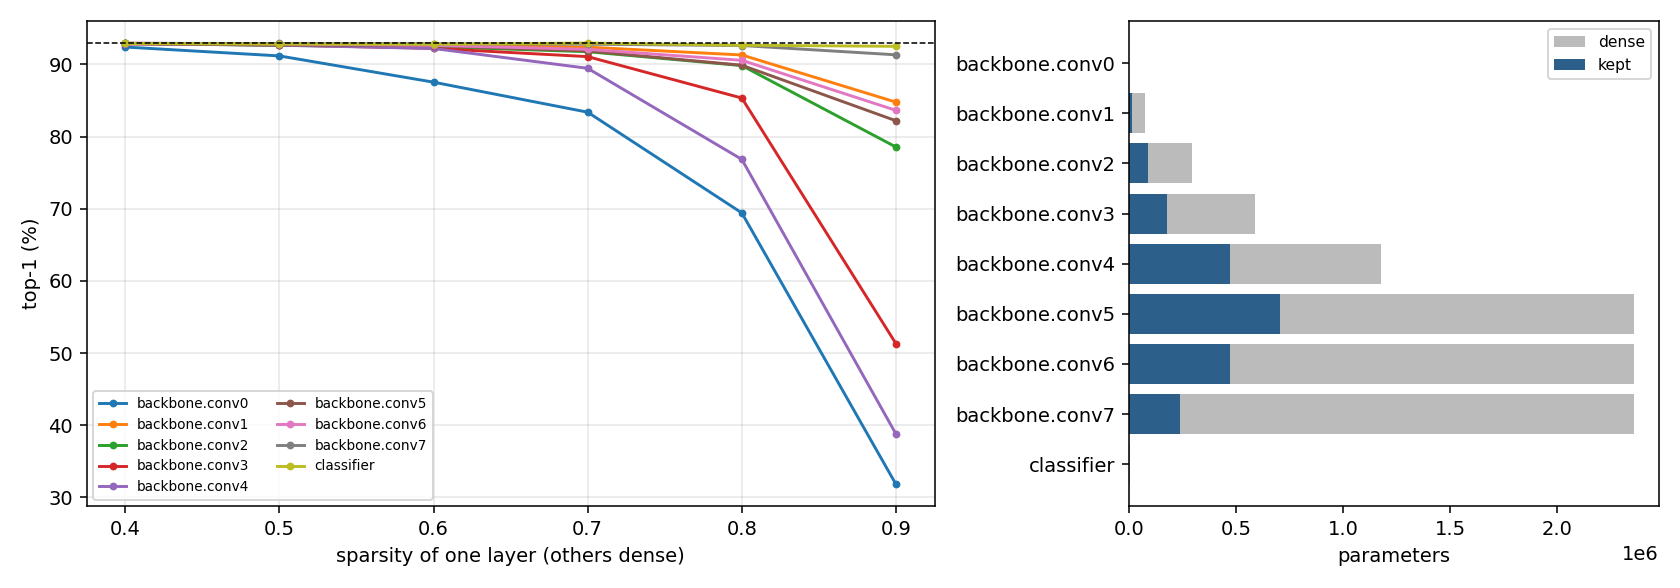
\includegraphics[width=\linewidth]{sensitivity.png}
\caption{左：逐层敏感度，把一层剪到横轴稀疏度、其余保持稠密时的准确率；虚线是稠密 92.95\%。右：每层稠密参数量（灰）与选定稀疏度后保留的参数量（蓝）。}\label{fig:sens}
\end{figure}

选稀疏度的规则：给每层同一个容许线 $\text{acc}_\text{dense}-d$，取准确率\emph{第一次}跌破容许线之前的最大稀疏度；$d$ 从 0 起每次加 0.1，取第一个使总尺寸 $\le 25\%$ 的 $d$。
本实验 $d=2.4$，得到 conv0--conv7 与 classifier 的稀疏度 0.5 / 0.8 / 0.7 / 0.7 / 0.6 / 0.7 / 0.8 / 0.9 / 0.9。
\Cref{fig:sens}右图说明了为什么 25\% 做得到：conv5--conv7 各有 236 万参数，占全部的 77\%，而它们恰好是最不敏感的几层；最敏感的 conv0 只有 1,728 个参数，剪多剪少对尺寸无影响。

\begin{table}[H]
\centering\small
\caption{细粒度剪枝（\texttt{lab1-pruning/artifacts/raw/summary.json}）}\label{tab:fg}
\begin{tabular}{lrr}
\toprule
阶段 & 准确率 & 尺寸 \\
\midrule
稠密 & 92.95\% & 35.20 MiB \\
剪枝后、微调前 & 78.39\% & 8.30 MiB（23.6\%） \\
微调第 1 / 2 / 3 / 4 / 5 轮 & 92.57 / 92.70 / 92.62 / 92.84 / 92.72\% & 8.30 MiB \\
\bottomrule
\end{tabular}
\end{table}

微调时每个 optimizer step 之后重新乘掩码，实测各层稀疏度与目标的偏差小于 $10^{-5}$。
细粒度稀疏不改变稠密 kernel 的计算量：单线程 9.25 $\to$ 9.18 ms（Xeon 8470Q），本地 Ice Lake 24.1 $\to$ 23.2 ms。

\subsection{通道剪枝}
\texttt{channel\_prune} 对除最后一个卷积外的每层保留前 $\mathrm{round}(c(1-r))$ 个输出通道，同步裁剪 BN 与下一层输入；最后一个卷积保持 512 通道，classifier 不变。
排序（\texttt{apply\_channel\_sorting}）用下一层权重对每个输入通道的 Frobenius 范数 $\|W^{(l+1)}_{:,j,:,:}\|_F$ 作为本层通道 $j$ 的重要性，按降序同步重排本层输出、BN 与下一层输入，函数不变（排序后 92.95\%）。

\begin{figure}[H]
\centering
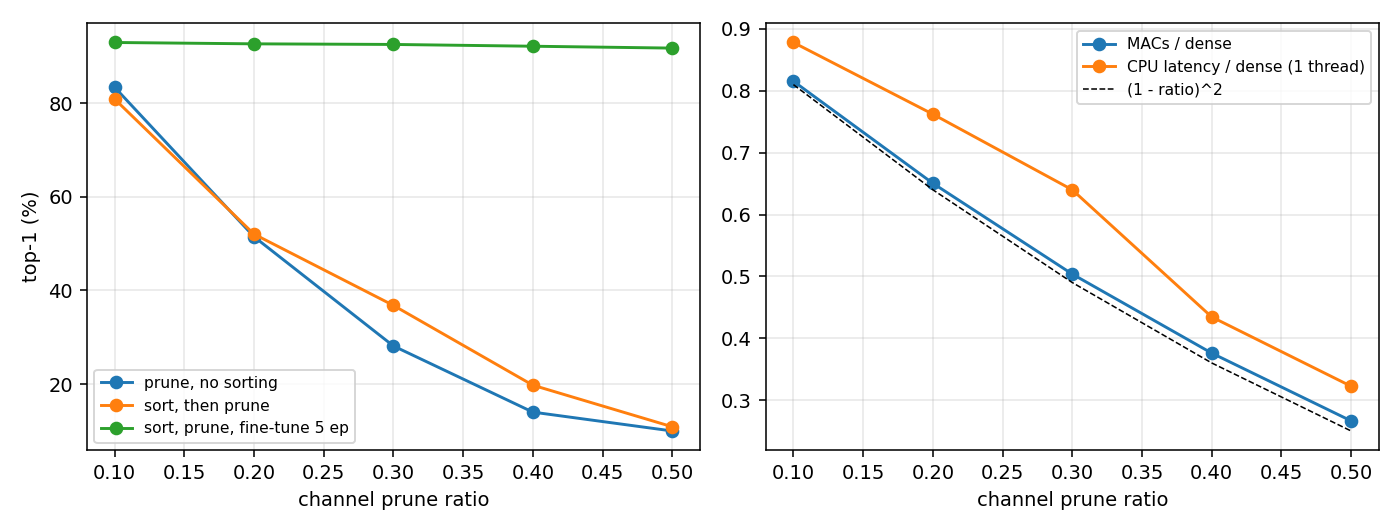
\includegraphics[width=\linewidth]{channel_pruning.png}
\caption{左：剪通道比例与准确率（不排序、排序、排序后微调 5 轮）。右：MACs 与单线程 CPU 延迟相对稠密的比值，虚线为 $(1-r)^2$。}\label{fig:ch}
\end{figure}

\begin{table}[H]
\centering\small
\caption{通道剪枝；延迟是 batch 1、单线程、p50}\label{tab:ch}
\begin{tabular}{rrrrrrr}
\toprule
比例 & 不排序 & 排序 & 排序+微调 & MACs & 延迟 8470Q & 延迟本地 \\
\midrule
0.1 & 83.40\% & 80.88\% & 92.94\% & 0.815 & 0.88 & 0.86 \\
0.2 & 51.48\% & 52.03\% & 92.65\% & 0.650 & 0.76 & 0.76 \\
0.3 & 28.15\% & 36.81\% & 92.52\% & 0.504 & 0.64 & 0.62 \\
0.4 & 14.03\% & 19.78\% & 92.14\% & 0.376 & 0.43 & 0.42 \\
0.5 & 10.00\% & 10.90\% & 91.74\% & 0.266 & 0.32 & 0.32 \\
\bottomrule
\end{tabular}
\end{table}

三点观察。第一，MACs 比几乎贴着 $(1-r)^2$：相邻两层的输入、输出通道都乘了 $1-r$；略高于它是因为第一层输入（3 通道）与最后一层输出（512）不剪。
第二，延迟比总高于 MACs 比（0.3 时 0.64 对 0.50），窄卷积里访存与调用开销所占比例更高；两台 CPU 的延迟比相差不到 0.02。
第三，排序只在剪得多时有用：$r=0.3$ 时不微调准确率从 28.15\% 升到 36.81\%，但 $r=0.1$ 时反而低 2.5 个点。输入通道范数只是对“这个通道被下一层用得多重”的粗略代理，没看本层激活的分布。

\begin{findingbox}[：Lab 1]
细粒度剪枝能把尺寸压到 23.6\% 而准确率不掉（92.72\%），但不会让稠密 kernel 变快；通道剪枝直接减 MACs，30\% 时延迟 0.64 倍、准确率 92.52\%。
要让细粒度稀疏变快，需要稀疏 kernel 或 2:4 这类硬件友好的结构。
\end{findingbox}

\section{Lab 2：k-means 量化与整数线性量化}\label{sec:lab2}

\subsection{k-means 权重共享与 QAT}
与 Deep Compression~\cite{deepcompression} 相同，每个卷积与线性层的权重单独聚成 $2^b$ 个中心。一维 Lloyd 迭代：分位数初始化，中心排序后用相邻中心的中点 \texttt{bucketize} 做最近中心分配（一维下这是精确的），最多 50 轮。
QAT 时标签固定，每个 optimizer step 后把每个中心移到“当前分到它的权重的均值”，再把权重写回中心值：
\begin{equation}
c_k \leftarrow \frac{1}{|\{i: \ell_i = k\}|}\sum_{i:\ell_i=k} w_i, \qquad w_i \leftarrow c_{\ell_i}.
\end{equation}
只有准确率比稠密低超过 0.5 点才微调，最多 5 轮，lr 0.01 按轮 cosine 衰减。

\begin{table}[H]
\centering\small
\caption{k-means 量化（\texttt{lab2-vgg/artifacts/raw/summary.json}）}\label{tab:km}
\begin{tabular}{rrrrr}
\toprule
位宽 & 直接量化 & QAT 后 & QAT 轮数 & 尺寸 \\
\midrule
32 & 92.95\% & — & — & 35.20 MiB \\
8 & 92.82\% & 92.82\% & 0 & 8.83 MiB \\
4 & 91.61\% & 92.84\% & 1 & 4.42 MiB \\
2 & 22.73\% & 92.18\% & 5 & 2.22 MiB \\
\bottomrule
\end{tabular}
\end{table}

2 bit 的 QAT 曲线是 91.97 / 92.20 / 92.16 / 92.15 / 92.18\%：第一轮就恢复了 69 个点，之后不再上升，仍比稠密低 0.77 点。每层只有 4 个值，第二轮以后中心只在小范围内移动。

\subsection{整数推理}
线性量化 $r = S(q - Z)$~\cite{jacob2018}。权重按输出通道对称（$Z=0$，$S=\max|w|/127$）；激活按张量非对称，用 512 张训练图的 min / max 标定；bias 量化为 int32，尺度 $S_xS_w$、零点 0。
输入预处理 $q=255x-128$ 对 8 bit 图片是精确的。BN 先融合进卷积：
\begin{equation}
W' = W\cdot\frac{\gamma}{\sqrt{\sigma^2+\epsilon}},\qquad b' = \beta + (b-\mu)\frac{\gamma}{\sqrt{\sigma^2+\epsilon}} .
\end{equation}
整数卷积为
\begin{equation}
q_y = \mathrm{clamp}\Bigl(\mathrm{round}\bigl(\tfrac{S_xS_w}{S_y}\bigl[\textstyle\sum (q_x - Z_x)\,q_w + q_b\bigr]\bigr) + Z_y,\ -128,\ 127\Bigr),
\end{equation}
padding 填输入零点（即真实值 0）。ReLU 不单独执行：输出在 ReLU 之后标定，min = 0，于是 $Z_y=-128$，clamp 的下限就是 ReLU。
GPU 上没有 int8 卷积，累加用 float64 模拟：本网络 $|\text{acc}|<2^{28}\ll 2^{53}$，结果与 int32 累加逐位相同。

\begin{table}[H]
\centering\small
\caption{整数推理（权重与激活同位宽，只做 PTQ）}\label{tab:lin}
\begin{tabular}{rrr}
\toprule
位宽 & 准确率 & 尺寸 \\
\midrule
fp32（融合 BN 后） & 92.95\% & 35.20 MiB \\
8 & 92.94\% & 8.82 MiB \\
6 & 92.75\% & 6.62 MiB \\
5 & 92.36\% & 5.52 MiB \\
4 & 89.98\% & 4.42 MiB \\
\bottomrule
\end{tabular}
\end{table}

\begin{figure}[H]
\centering
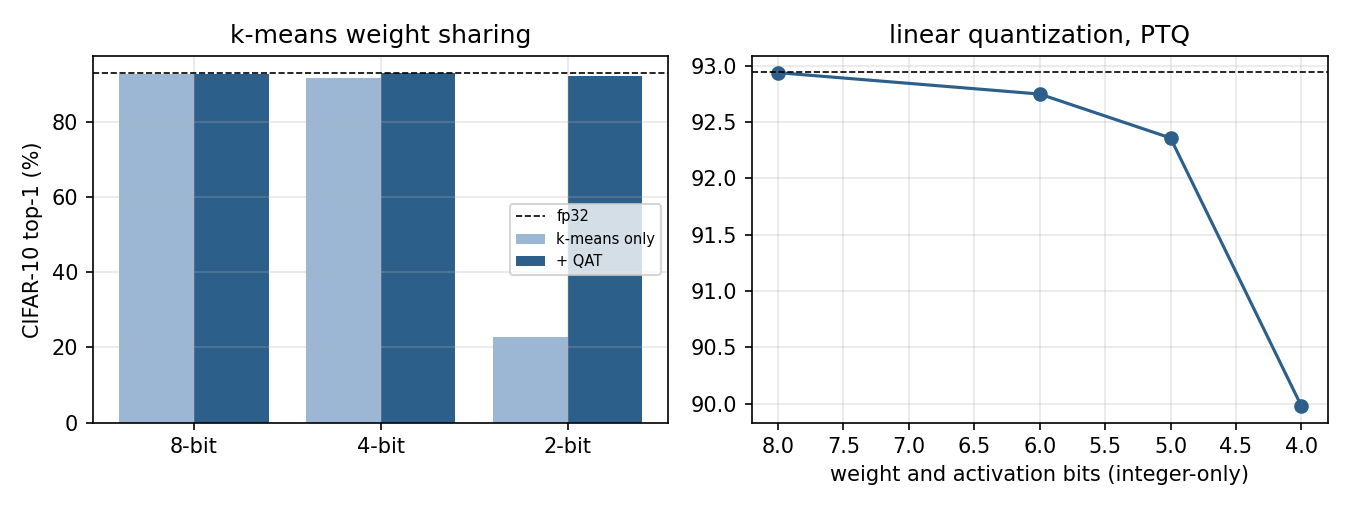
\includegraphics[width=0.95\linewidth]{lab2_vgg.png}
\caption{左：k-means 量化，直接量化与 QAT 后；右：整数线性量化的位宽扫描。}\label{fig:lab2}
\end{figure}

\begin{findingbox}[：Lab 2]
同为 4 bit、同样 4.42 MiB，k-means 经一轮 QAT 是 92.84\%，整数线性 PTQ 是 89.98\%：非均匀码本更贴近权重分布，但推理时要查表解码，换不来整数算力。
8 bit 时两者都与 fp32 几乎相同，整数版本层间全是 int8，可以直接映射到 CMSIS-NN / TFLM 的 int8 kernel。
\end{findingbox}

\section{Lab 4：OPT-1.3B 上的 AWQ}\label{sec:lab4}

\subsection{协议}
\texttt{facebook/opt-1.3b} fp16。困惑度：wikitext-2-raw test 拼接后前 $40\times2048$ 个 token；校准：pile-val 前 128 条长度不超过 512 token 的文本，拼接后切成 59 个 512 token 块。
伪量化：每 128 个输入维一组，按组 min / max 非对称，$S=(\max-\min)/(2^b-1)$，$Z=-\mathrm{round}(\min/S)$；量化后写回 fp16 计算。

\subsection{显著通道与缩放搜索}
Q1：整体量化后把重要性最高的 $k$ 个输入列写回原值。重要性有三种：激活 $\overline{|x_j|}$、权重 $\overline{|W_{:,j}|}$、随机。
Q2（AWQ~\cite{awq}）：对共享同一输入的一组 linear，搜
\begin{equation}
\alpha^\star = \arg\min_{\alpha\in\{0,0.05,\dots,0.95\}} \bigl\| Q\bigl(W\,\mathrm{diag}(s)\bigr)\,\bigl(\mathrm{diag}(s)^{-1}x\bigr) - Wx \bigr\|^2,\qquad s = s_x^{\alpha},
\end{equation}
$\alpha=0$ 就是 RTN。$1/s$ 折进上游：q/k/v 折进 \texttt{self\_attn\_layer\_norm}，out\_proj 折进 v\_proj 的输出行，fc1 折进 \texttt{final\_layer\_norm}，fc2 折进 fc1 的输出行（ReLU 正齐次）。
截断搜索对每组取阈值 $\max|w|\cdot r$，$r\in\{1,0.95,\dots,0.55\}$，按该组对输出的误差选；q/k 不截断。

\begin{table}[H]
\centering\small
\caption{OPT-1.3B，group 128（\texttt{lab4-awq/artifacts/raw/summary.json}）}\label{tab:awq}
\begin{tabular}{lrrr}
\toprule
方法 & 位宽 & 困惑度 & 尺寸 \\
\midrule
FP16 & 16 & 14.47 & 2509.6 MiB \\
RTN & 3 & 107.97 & 659.0 MiB \\
1\% fp16，按激活 & 3 & 16.69 & 677.5 MiB \\
1\% fp16，按权重 & 3 & 103.41 & 677.5 MiB \\
1\% fp16，随机 & 3 & 106.79 & 677.5 MiB \\
0.1\% / 3\% fp16，按激活 & 3 & 17.39 / 16.57 & 660.8 / 714.5 MiB \\
AWQ & 3 & 16.87 & 659.0 MiB \\
AWQ + 截断 & 3 & \textbf{16.04} & 659.0 MiB \\
RTN & 4 & 15.08 & 804.1 MiB \\
AWQ / AWQ + 截断 & 4 & \textbf{14.78} / 14.80 & 804.1 MiB \\
\bottomrule
\end{tabular}
\end{table}

\begin{figure}[H]
\centering
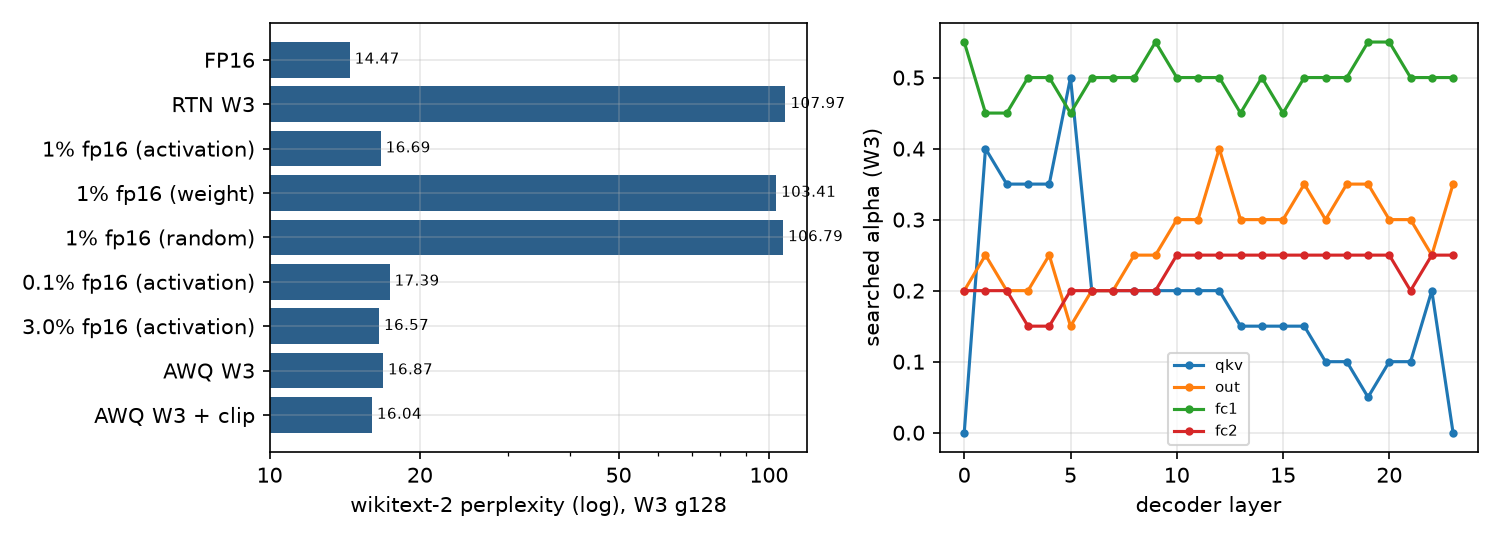
\includegraphics[width=0.95\linewidth]{awq_opt1.3b.png}
\caption{左：W3 g128 的困惑度（对数轴）。右：每层搜到的 $\alpha$。}\label{fig:awq}
\end{figure}

\Cref{tab:awq} 的关键对照是同为“保留 1\%”的三行：按激活 16.69，按权重 103.41，随机 106.79。显著性来自激活幅度，大权重并不重要。
保留 0.1\% 就已经到 17.39，再多到 3\% 只到 16.57：少数几个离群通道贡献了绝大部分误差。
AWQ 把“保留”换成“放大再量化”：放大 $s$ 倍的通道相对量化误差缩小，而 $1/s$ 在上游以 fp16 吸收，所以不需要混合精度存储，尺寸与 RTN 相同。
搜到的 $\alpha$（\cref{fig:awq} 右）：fc1 稳定在 0.45--0.55，fc2 在 0.15--0.25，qkv 随层加深从 0.35--0.5 降到 0.05--0.2。
4 bit 时截断不再有用（14.78 对 14.80）：组内 16 级已经够细，截断带来的离群值误差大于它省下的舍入误差。

\begin{iqbox}{为什么 AWQ 按激活而不是按权重判断重要性？}
量化误差对输出的贡献是 $\Delta W_{:,j}\,x_j$：同样的权重误差乘上大的 $|x_j|$ 才放大。本实验按权重幅度保留 1\% 列困惑度 103.41，几乎等于不保留（107.97）；按激活保留 16.69。
所以“重要”是输入通道的性质，而一个输入通道对应 $W$ 的一列，缩放整列不改变函数，可以把 $s$ 折进上一层，这是 AWQ 不需要混合精度的原因。
\end{iqbox}

\section{Lab 5：W4A8 GEMM kernel 与 LLaMA2-7B}\label{sec:lab5}

\subsection{设置}
tinychat-tutorial（commit \texttt{f241215}）里 TinyChatEngine 的 \texttt{QM\_x86} 格式：每 32 字节存 64 个 4 bit 权重，字节 $j$ 的低 4 位是权重 $j$、高 4 位是权重 $j+32$，以 $w+8$ 存；每 32 个权重一个 fp32 scale，激活每 32 个一个 int8 scale。模型是 AWQ~\cite{awq} 量化的 LLaMA2-7B-chat。
改动只在 \texttt{kernels/starter\_code/} 的五个文件里（110 行新增，x86 与 NEON 两条分支）。主机 Xeon Platinum 8470Q，g++ 11.4，课程 Makefile 原样（\texttt{-O0 -mavx2 -mfma}）；kernel 基准用 \texttt{taskset} 限 8 核，端到端限另外 6 核。

\subsection{四种技术}
展开：一次解码 4 个字节，累加器拆两路。多线程：按输出列切成 \texttt{num\_thread} 段，pthread create / join；与展开合用时段长取 4 的倍数。
SIMD：\texttt{and 0x0F} 与 \texttt{srli 4} 拆半字节，\texttt{sub 8} 回到有符号，然后
\begin{equation}
\textstyle\sum_j w_j a_j = \texttt{madd\_epi16}\bigl(\texttt{maddubs\_epi16}(|w|,\ \mathrm{sign}(a, w)),\ 1\bigr),
\end{equation}
\texttt{maddubs} 只接受“无符号 $\times$ 有符号”，所以把 $w$ 的符号挪到 $a$ 上。这一步在 $a=-128$、$w<0$ 时出错：$-(-128)$ 在 int8 里仍是 $-128$。引擎的激活量化用 $\max|a|/127$，激活落在 $[-127,127]$，不触发；测试把 16 个权重值与 256 个激活值的组合全部枚举，错误恰好只出现在这一处。
全部技巧：SIMD 每次处理两个 32 字节块，8 线程。

\begin{table}[H]
\centering\small
\caption{W4A8 kernel：test\_linear 是 $1\times4096\times4096$ GEMV，端到端是 decode 第 2--32 个 token 的平均（\texttt{lab5-tinychat/artifacts/raw/summary.json}）}\label{tab:lab5}
\begin{tabular}{lrrrrrr}
\toprule
 & \multicolumn{4}{c}{\texttt{-O0}（课程）} & \multicolumn{2}{c}{\texttt{-O3}} \\
\cmidrule(lr){2-5}\cmidrule(lr){6-7}
kernel & GOP/s & 倍数 & ms/token & 倍数 & GOP/s & 倍数 \\
\midrule
reference & 0.93 & 1.0 & 14427 & 1.0 & 4.33 & 1.0 \\
loop\_unrolling & 1.87 & 2.0 & 6998 & 2.1 & 10.85 & 2.5 \\
multithreading（4 线程） & 3.34 & 3.6 & 4417 & 3.3 & 14.49 & 3.4 \\
simd\_programming & 2.53 & 2.7 & 5654 & 2.6 & 48.90 & 11.3 \\
mt + unrolling（4 线程） & 6.78 & 7.3 & 2252 & 6.4 & 40.46 & 9.4 \\
all\_techniques（8 线程） & \textbf{26.09} & \textbf{28.2} & \textbf{1150} & \textbf{12.5} & \textbf{222.70} & \textbf{51.5} \\
\bottomrule
\end{tabular}
\end{table}

\begin{figure}[H]
\centering
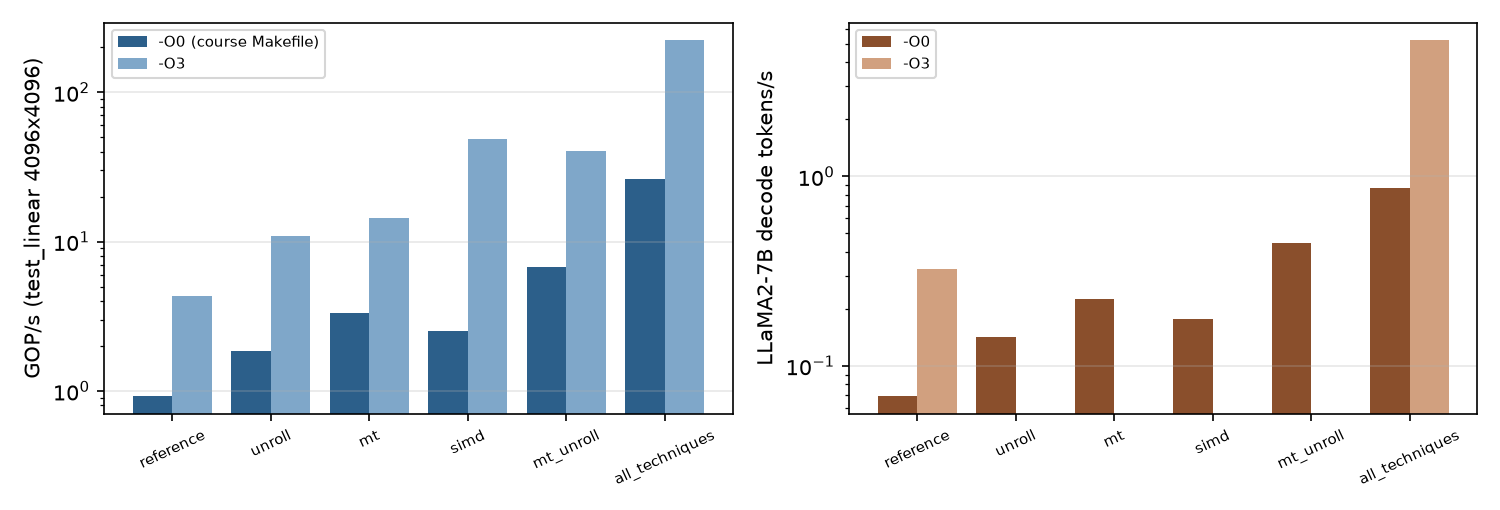
\includegraphics[width=\linewidth]{lab5_kernels.png}
\caption{左：test\_linear 的 GOP/s（对数轴），\texttt{-O0} 与 \texttt{-O3}。右：LLaMA2-7B decode 的 token/s；\texttt{-O3} 只测了首尾两个实现（191 与 3085 ms/token）。}\label{fig:lab5}
\end{figure}

两点观察。第一，前四个实现端到端的倍数与 kernel 倍数基本一致（2.1--6.4 对 2.0--7.3），说明 \texttt{-O0} 下 decode 几乎全花在 GEMV 上；\texttt{all\_techniques} kernel 快 28.2 倍，端到端只快 12.5 倍，剩下的时间在注意力、RMSNorm 这些没改过的算子上。
第二，\texttt{-O0} 低估了手写 SIMD：\texttt{-O3} 下参考实现快了 4.7 倍，\texttt{all\_techniques} 快了 8.5 倍；单线程 SIMD（48.9）反超 4 线程展开（40.5），编译器能优化标量循环，但做不出 \texttt{maddubs} 这样跨 lane 的成对乘加。

\begin{findingbox}[：Lab 5]
手写 AVX2 + 8 线程把 4096 方阵的 W4A8 GEMV 做到 222.7 GOP/s（\texttt{-O3}，参考实现的 51.5 倍），7B 模型 decode 5.2 token/s；kernel 越快，没改过的算子在端到端里占比越高。
符号挪移技巧依赖“激活不取 $-128$”这一契约，它写在量化器里而不在 kernel 里；换一个按 $\max|a|/128$ 量化的前端，kernel 会静默算错。
\end{findingbox}

\begin{thebibliography}{99}
\bibitem{han2015} S.~Han, J.~Pool, J.~Tran, W.~J.~Dally. Learning both Weights and Connections for Efficient Neural Networks. \emph{NeurIPS}, 2015.
\bibitem{deepcompression} S.~Han, H.~Mao, W.~J.~Dally. Deep Compression: Compressing Deep Neural Networks with Pruning, Trained Quantization and Huffman Coding. \emph{ICLR}, 2016.
\bibitem{jacob2018} B.~Jacob, S.~Kligys, B.~Chen, M.~Zhu, M.~Tang, A.~Howard, H.~Adam, D.~Kalenichenko. Quantization and Training of Neural Networks for Efficient Integer-Arithmetic-Only Inference. \emph{CVPR}, 2018.
\bibitem{awq} J.~Lin, J.~Tang, H.~Tang, S.~Yang, W.-M.~Chen, W.-C.~Wang, G.~Xiao, X.~Dang, C.~Gan, S.~Han. AWQ: Activation-aware Weight Quantization for On-Device LLM Compression and Acceleration. \emph{MLSys}, 2024.
\end{thebibliography}

\end{document}
